\begin{figure}[h]
	\centering
	\missingfigure{Klassendiagramm}		
	\caption{Klassendiagramm - A}
	\label{fig:klassendiagramm-a}
\end{figure}

\begin{table}[h]
	\centering
	\begin{tabularx}{\textwidth}{X X}
		\rowcolor[HTML]{C0C0C0} 
		\textbf{Klassenname} & \textbf{Aufgabe} \\
		Klasse A & Aufgabe A \\
		\rowcolor[HTML]{E7E7E7} 
		Klasse B & Aufgabe B \\
		Klasse C & Aufgabe C \\
		\rowcolor[HTML]{E7E7E7} 
		Klasse D & Aufgabe D \\
		Klasse E & Aufgabe E \\
		\rowcolor[HTML]{E7E7E7} 
		Klasse F & Aufgabe F \\
		Klasse G & Aufgabe G
	\end{tabularx}
	\caption{Klassenbeschreibung - A}
	\label{table:klassenbeschreibung-a}
\end{table}

\begin{tcolorbox}
Teilt eure Klassendiagramme bitte auf und baut \textbf{kein} einzelnes riesiges Diagramm.
Getter und Setter Methoden müssen hier nicht modelliert werden.
Sie sollten aber der klassischen Namenskonvention folgen, um die Nutzung in Sequenzdiagrammen zu ermöglichen.
\\\\
Auf jedes Diagramm folgt eine Tabelle, in der die Aufgabe \textbf{jeder} Klasse beschrieben wird.
\end{tcolorbox}

\begin{figure}[h]
	\hspace{-3cm}
	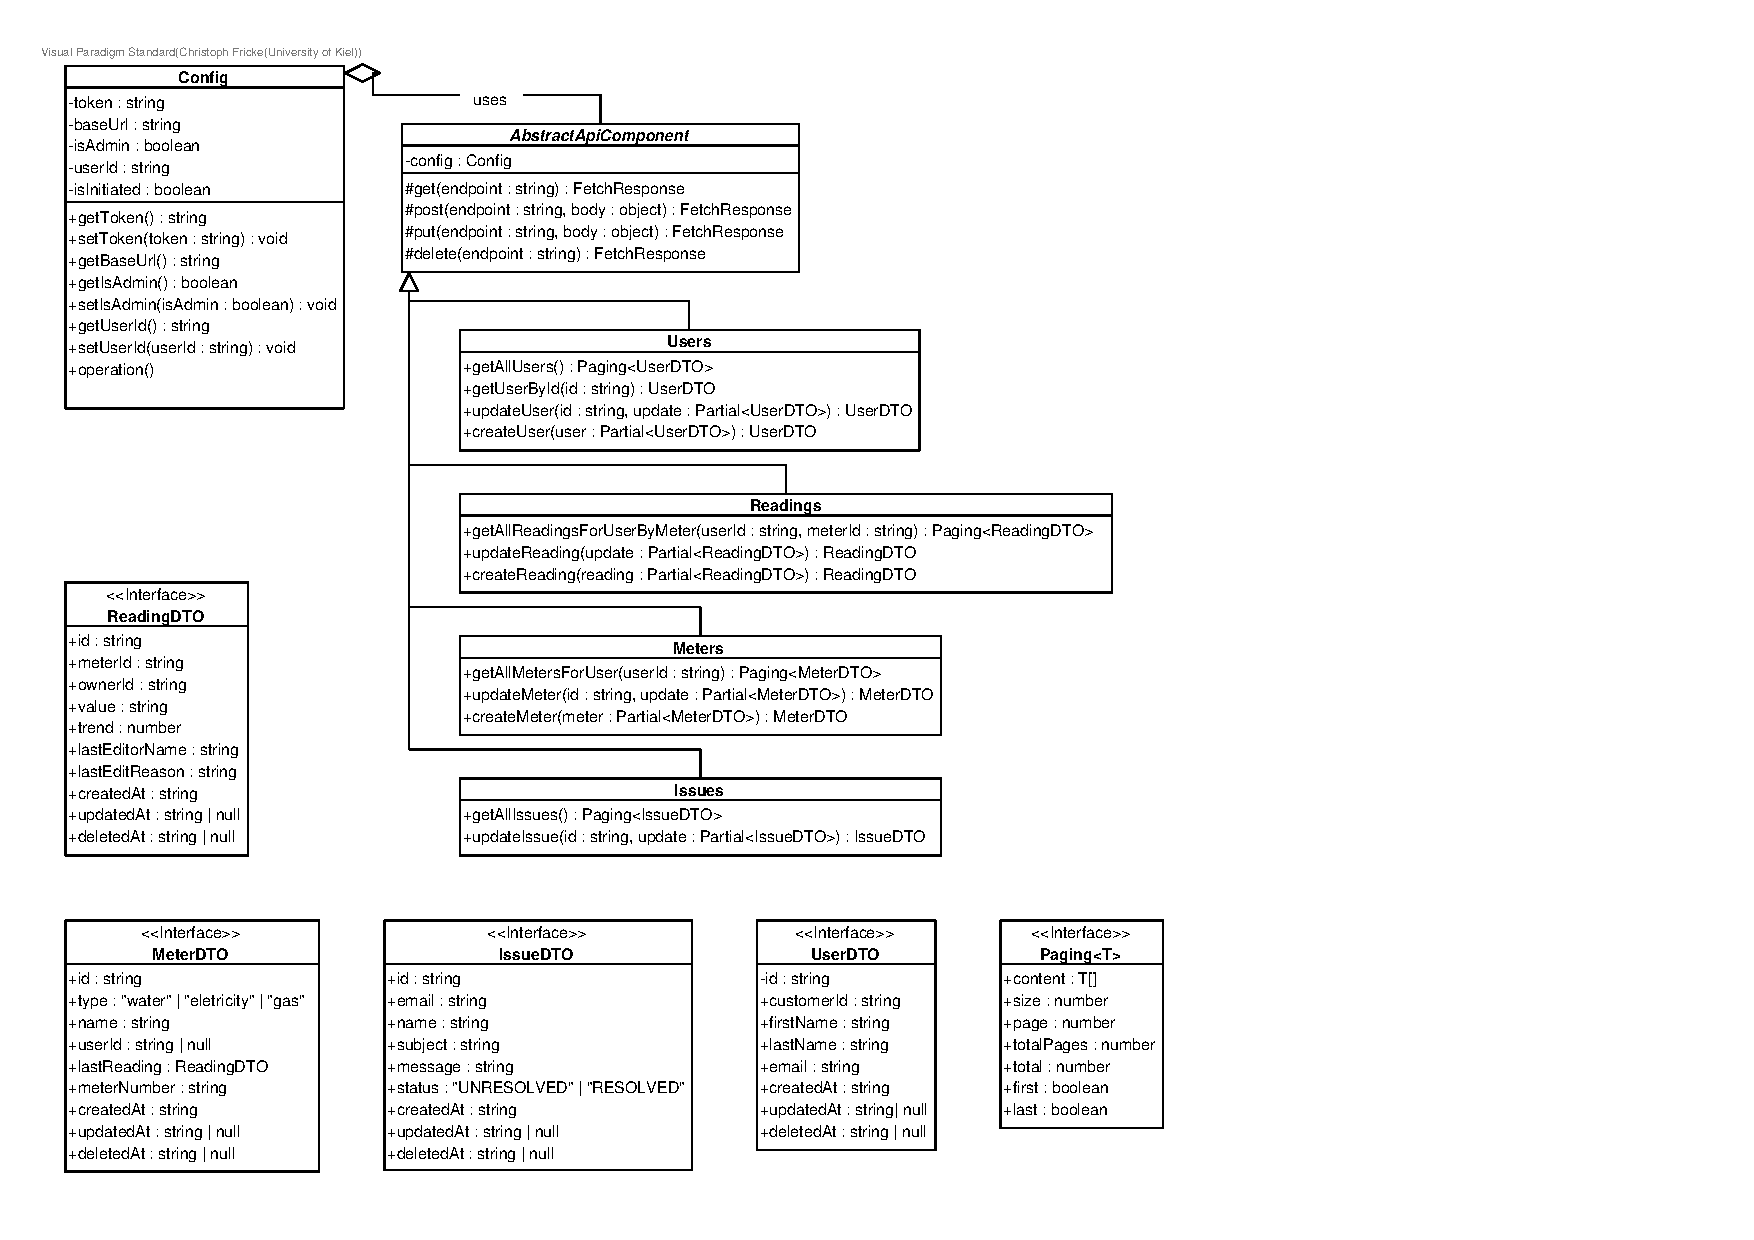
\includegraphics{./img/Diagrams/api-classDiagram}
\end{figure}

\begin{figure}[h]
	\hspace{-3cm}
	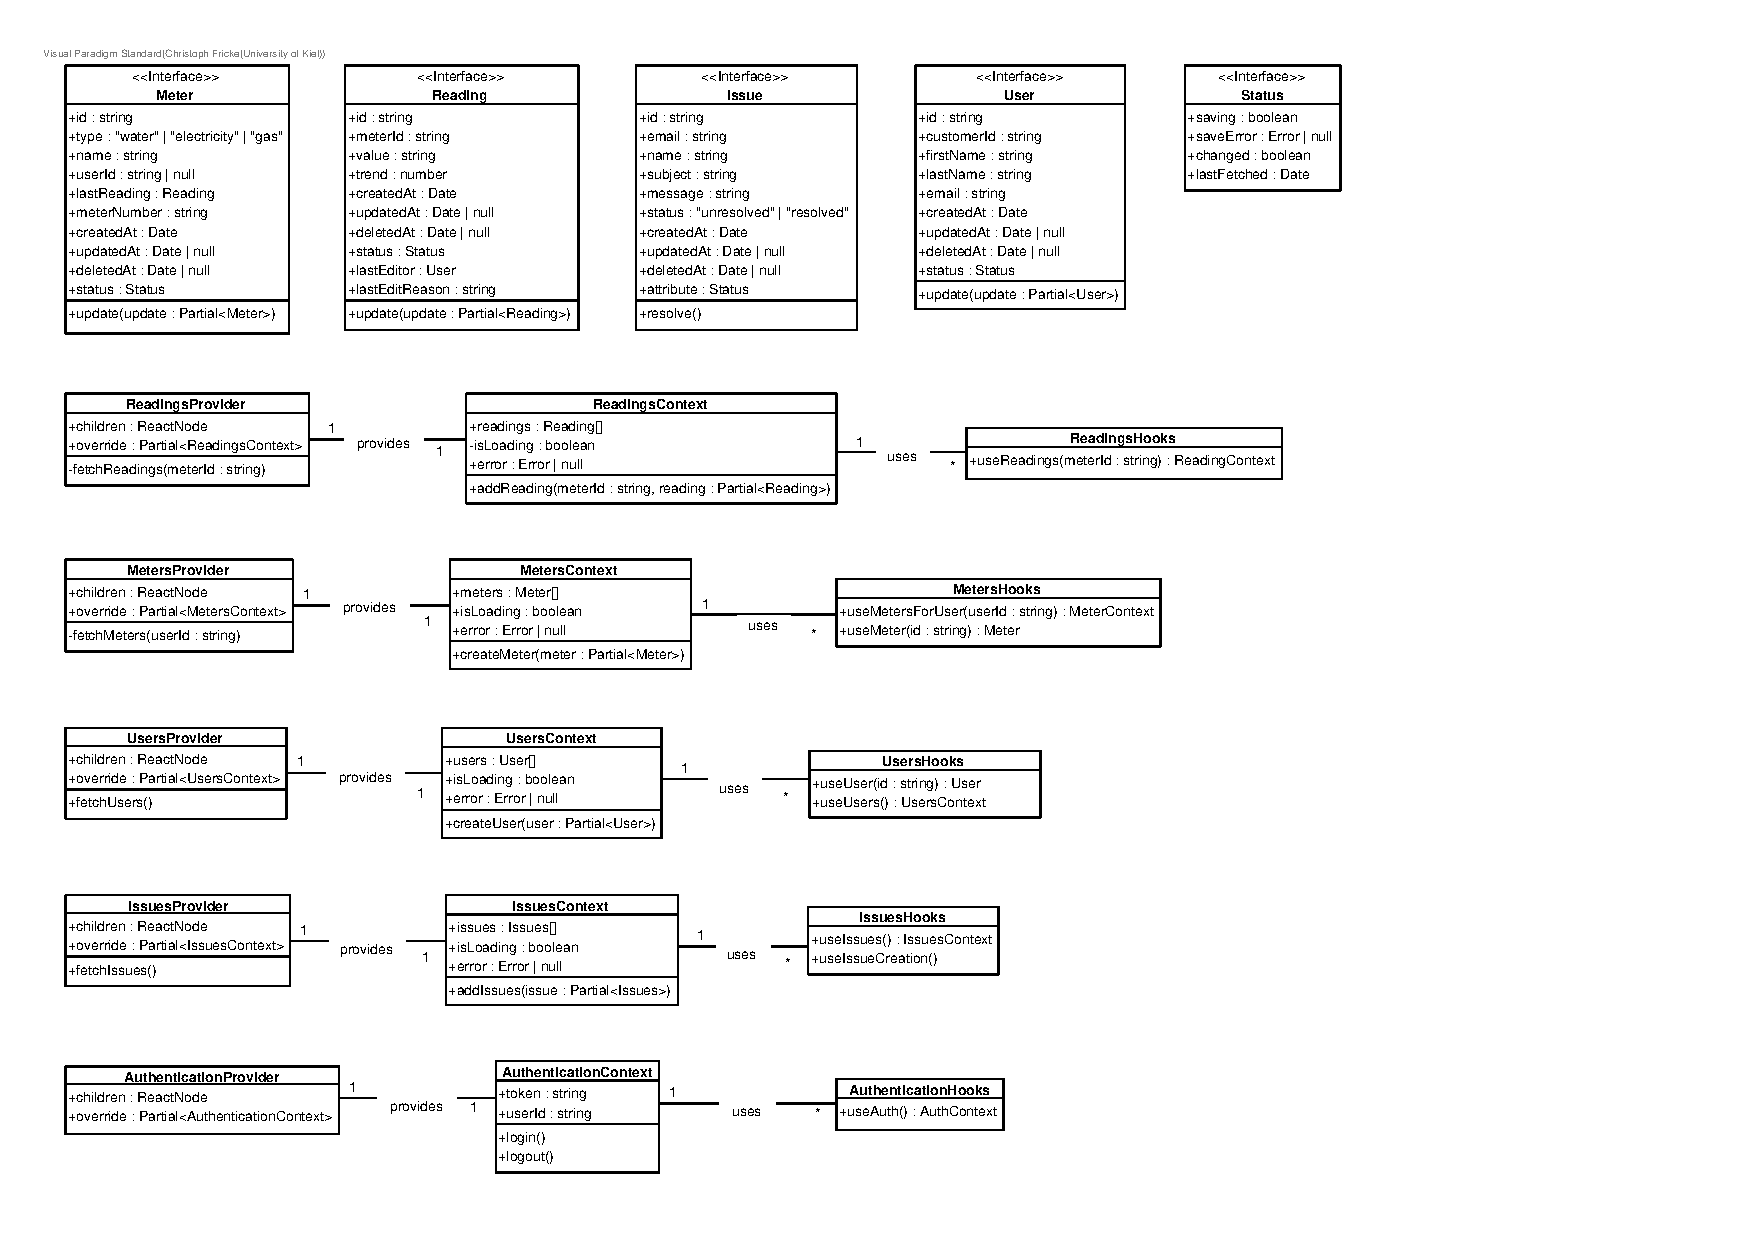
\includegraphics[scale = 0.9]{./img/Diagrams/providers-classDiagram}
\end{figure}

\begin{figure}[h]
	\hspace{-3cm}
	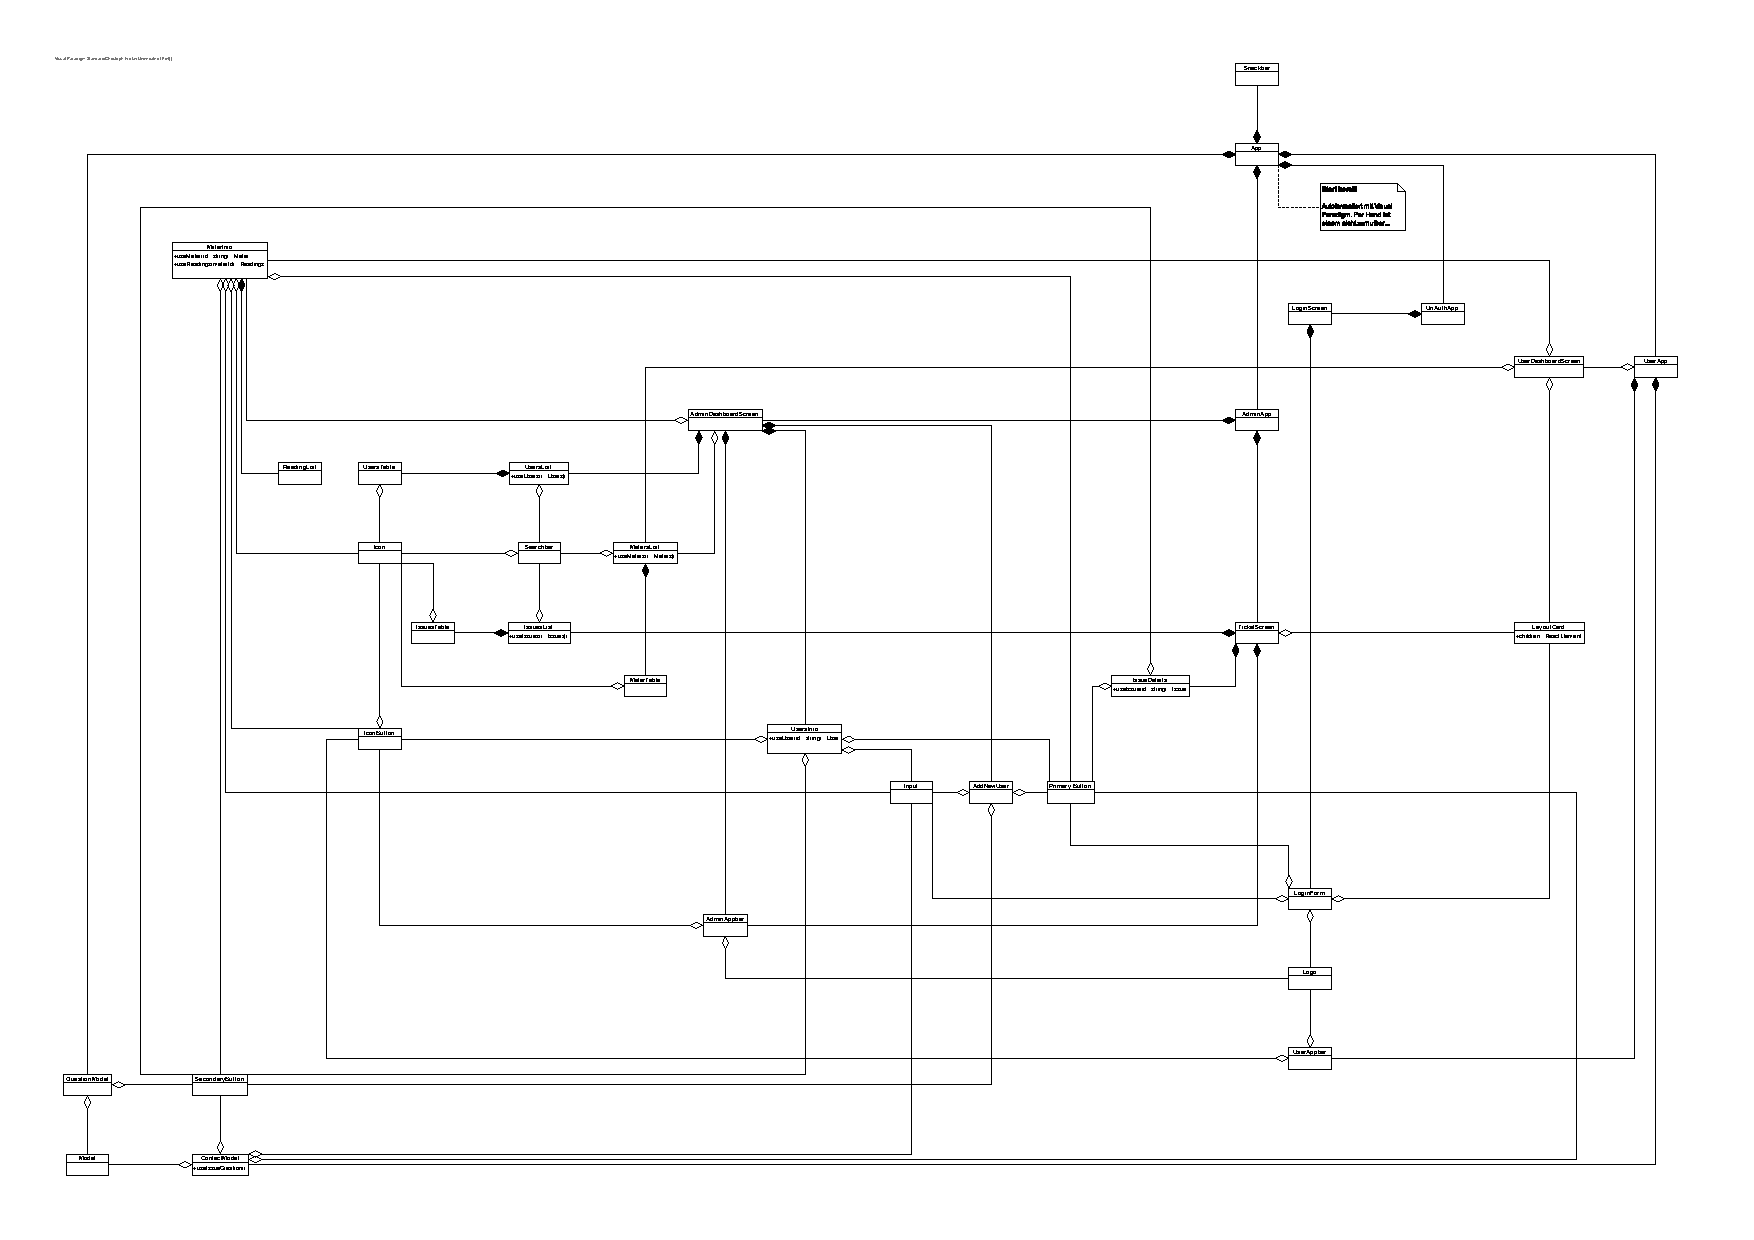
\includegraphics[scale = 0.73]{./img/Diagrams/web-class}
\end{figure}